\chapter{Percolation}
\label{ch:percolation}

Percolation on a chygraph was solved by
\citet{vazquez2023pre,vazquez2024comnet}, and this chapter is the account
of it. It comes first among the applications because percolation is the case in
which the message travelling along an inclusion is a single number, a point
Chapter~\ref{ch:statmech} makes precise. Everything harder in this book is the
same recursion carrying something heavier.

The chapter's main claim is about labour rather than physics. The higher-order network literature has produced a separate percolation
calculation for hypergraphs, for multiplex networks, for interacting networks,
for simplicial complexes and for graphs with motifs, and the derivations have
been multiplying faster than anyone can hold them in one head
\citep{battiston2020,bianconi2021}. All of those structures are chygraphs
(Sec.~\ref{sec:everything}). So there is one calculation, and each published
result is recovered by writing down four small matrices and substituting.
Sections~\ref{sec:map} and~\ref{sec:threshold} give the calculation;
Sec.~\ref{sec:structurebystructure} does the substituting.

Section~\ref{sec:helporhurt} is not in the papers. It settles whether triangles
help percolation or hurt it, a question Eq.~\eqref{eq:thetaNM} raises and
Chapter~\ref{ch:ising} appears to answer the other way.

\section{Percolation on a chygraph}
\label{sec:percolation-chygraph}

Standing at a complex there are two ways out (Sec.~\ref{sec:vocabulary}): up,
through a complex that includes it, and down, into the complexes it includes.
Following those steps repeatedly from a starting complex reaches some subset of
the chygraph, and that subset is a \emph{component}. A \emph{giant component} is
one containing a finite fraction of the complexes as the chygraph grows.

Because layers are distinct kinds of object, the natural order parameter is not
one number but one per layer: $S_{l}$, the fraction of layer-$l$ complexes in
the giant component. When the chygraph is a graph and layer $0$ is its nodes,
$S_{0}$ is the ordinary giant component fraction, and $S\equiv S_{0}$ throughout
the book.

The question is when $S$ becomes positive, and how large it is once it has.

\section{The map}
\label{sec:map}
\index{self-consistency map|textbf}
\index{percolation!on a chygraph|textbf}

Everything follows from asking a question about one inclusion at a time, in the
manner of Sec.~\ref{sec:percolation-intro}, with two complications that the
graph case does not have: a step can go up or down, and the complex arrived at
has a layer.

So let $Q^{ml}_{i}$ be the probability that a layer-$l$ complex, reached from a
layer-$m$ complex, is \emph{not} connected to the giant component by any route
other than the one used to arrive. The index $i$ records the direction of
arrival: $i=-$ means the complex was reached from below, from a complex it
includes, and $i=+$ from above, from a complex that includes it. There are
$2L^{2}$ of these quantities, which sounds like a lot and is in fact the entire
state of the calculation however large the complexes are.

To be not connected, a complex must fail to connect through \emph{every} onward
route --- through each complex that includes it, and through each complex inside
it. Since the generating function of a distribution evaluated at a probability
is exactly the average of that probability raised to the number of routes, the
two conditions read
\begin{align}
  Q^{ml}_{-}&=\prod_{k}\Phi^{l}_{k}\bigl(Q^{lk}_{-}\bigr)
              \prod_{k}\bigl[\bar G^{l}_{k}\bigr]_{k=m}\bigl(Q^{lk}_{+}\bigr),
  \label{eq:Qminus}\\
  Q^{ml}_{+}&=\prod_{k}\bigl[\bar\Phi^{l}_{k}\bigr]_{k=m}\bigl(Q^{lk}_{-}\bigr)
              \prod_{k}G^{l}_{k}\bigl(Q^{lk}_{+}\bigr),
  \label{eq:Qplus}
\end{align}
with $\Phi$ and $G$ the generating functions of Sec.~\ref{sec:ensembles} --- up
through the chy-degree and down through the intra-complex component --- and
$[\bar F]_{k=m}$ meaning the excess function when $k=m$ and the ordinary one
otherwise.

That last piece of notation carries an idea. Arriving
somewhere along a link, one must not count that link again as a way onward: this
is the excess degree of Eq.~\eqref{eq:excessdeg}, and it is why $\bar\Phi$
rather than $\Phi$ appears. But on a chygraph one arrives from a \emph{layer},
and the step used to arrive has to be discounted only from the routes back into
that same layer. Routes into other layers were never available along it and are
counted in full. Hence the bracket: excess when the return layer $k$ equals the
layer of origin $m$, ordinary otherwise. On a graph, where there is only one
layer to go back to, this collapses to the familiar rule and disappears from
view.

The direction index follows the step and needs no bookkeeping of its own: a step
upward through a chy-degree lands in a $-$ state, a step downward through an
intra-complex component lands in a $+$ state.

\begin{figure}[t]
\centering
\begin{adjustbox}{max width=0.95\linewidth}
\begin{tikzpicture}
% the complex under consideration; layers are named inside the boxes so that no
% label has to compete with the arrows for space
\node[cpx,minimum size=4.6mm,font=\tiny] (E) at (0,0) {$l$};
% up: the complexes that include it
\node[cpx] (u1) at (-1.75,1.55) {}; \node[cpx] (u2) at (0,1.55) {};
\node[cpx] (u3) at (1.75,1.55) {};
\draw[msg] (-0.20,0.28) -- (-1.55,1.32);
\draw[msg] (0,0.30) -- (0,1.32);
\draw[msg] (0.20,0.28) -- (1.55,1.32);
\node[lb,anchor=south,align=center] at (0,1.92)
  {\emph{up}, through $\Phi^{l}_{k}$: each gives $Q^{lk}_{-}$};
% down: the complexes inside it
\node[atm] (d1) at (-1.35,-1.75) {}; \node[atm] (d2) at (0,-1.75) {};
\node[atm] (d3) at (1.35,-1.75) {};
\draw[msg] (-0.18,-0.30) -- (-1.18,-1.52);
\draw[msg] (0,-0.32) -- (0,-1.52);
\draw[msg] (0.18,-0.30) -- (1.18,-1.52);
\node[lb,anchor=north,align=center] at (0,-2.10)
  {\emph{down}, through $G^{l}_{k}$: each gives $Q^{lk}_{+}$};
% the arrival, and what it excludes
\node[cpx,minimum size=4.6mm,font=\tiny] (arr) at (-3.45,0) {$m$};
\draw[lnk,line width=1.1pt] (arr)--(E);
\node[lb,anchor=south] at (-1.72,0.10) {arrived};
\node[lb,anchor=west,align=left] at (2.55,0)
  {the arriving step is\\ discounted only from\\ routes back into\\ layer $m$};
\end{tikzpicture}
\end{adjustbox}
\caption{\textbf{The map.} A complex reached from layer $m$ fails to reach the
giant component only if every onward route fails --- every complex that includes
it and every complex inside it. Equations~\eqref{eq:Qminus}
and~\eqref{eq:Qplus} are that statement, one for each direction of arrival. The
only subtlety is the one on the right: the inclusion used to arrive must not be
counted again, but it was only ever a route back into layer $m$, so the excess
generating function is used for that layer and the ordinary one for every other.}
\label{fig:themap}
\end{figure}

Solving Eqs.~\eqref{eq:Qminus}--\eqref{eq:Qplus} --- by iteration from
$Q\equiv0$, which converges to the relevant fixed point --- gives everything.
The probability that a randomly chosen layer-$l$ complex is in no giant
component is the same statement made at a complex rather than along an
inclusion, so with no excess anywhere,
\begin{equation}
  P^{l}=\prod_{k}\Phi^{l}_{k}\bigl(Q^{lk}_{-}\bigr)
        \prod_{k}G^{l}_{k}\bigl(Q^{lk}_{+}\bigr),
  \qquad S_{l}=1-P^{l}.
  \label{eq:Sl}
\end{equation}

\paragraph{Occupation probabilities.} Site and bond occupation enter by
\emph{thinning} the generating functions rather than as a separate calculation:
a complex present with probability $p$ sends $\Phi\to1-p+p\Phi$. This makes
$S_{l}$ the fraction of \emph{all} layer-$l$ complexes rather than of surviving
ones, so that $S\le p$ automatically.

Thinning is not always the right move, and Chapter~\ref{ch:giant} turns on the
exception. When the connectivity rule already
implies that a complex is present --- as under AND-logic, where a hyperedge
functions only if all its members do --- a complex reached along a working
inclusion is present by construction, and folding the occupation probability
into the map would count it twice. It is then reinstated at the root only,
$P^{l}\to1-\pi_{l}+\pi_{l}P^{l}$.

\section{The threshold}
\label{sec:threshold}
\index{threshold tensor|textbf}

The map always has the trivial fixed point $Q\equiv1$: nothing is connected to
anything. A giant component exists exactly when that fixed point is unstable,
which is the chygraph version of the branching argument of
Sec.~\ref{sec:percolation-intro} --- one branch begetting more than one branch.

Linearising Eqs.~\eqref{eq:Qminus}--\eqref{eq:Qplus} about $Q\equiv1$ replaces
every generating function by its first derivative there, which by
Eq.~\eqref{eq:moments} is one of the four moment matrices $\ave{\kappa}$,
$\ave{\kbar}$, $\ave{s}$, $\ave{\sbar}$. The result is a linear operator on the
$2L^{2}$ unknowns --- the tensor $A$ of \citet{vazquez2023pre} --- and the
transition is where the largest eigenvalue of $-A$ passes through zero. The
sign is not cosmetic. Section~\ref{sec:jacobian} will show that $A$ is the
identity minus the Jacobian of the map, so its eigenvalues are the Jacobian's
subtracted from one, and the one that crosses zero at the transition is the
smallest of them rather than the largest.

Doing that expansion is what produces the blocks. Write $Q=1-\epsilon$. Every
generating function equals one at $Q\equiv1$, so a product of them is one at
zeroth order and each factor contributes nothing but its own first derivative,
\[
  \prod_{k}\Phi^{l}_{k}\bigl(1-\epsilon^{lk}_{-}\bigr)
    =1-\sum_{k}\ave{\kappa}_{lk}\,\epsilon^{lk}_{-}+O(\epsilon^{2}),
\]
and the same for $\bar\Phi$, $G$ and $\bar G$ with $\ave{\kbar}$, $\ave{s}$ and
$\ave{\sbar}$. The two products in each of Eqs.~\eqref{eq:Qminus}
and~\eqref{eq:Qplus} multiply, and to first order their corrections simply add,
so each equation becomes one row reading $\epsilon^{ml}_{\pm}$ against a sum of
moments times $\epsilon^{lk}_{-}$ and $\epsilon^{lk}_{+}$. Collecting every term
on one side gives $A\epsilon=0$, the identity piece below being the left-hand
side of that row and the moments what it is set equal to.

Index the four blocks of $A$ by the direction of arrival at the complex and the
direction of departure from it. With $\delta$ the Kronecker delta,
\begin{align*}
  (A_{--})^{ml}_{nk}&=\delta_{mn}\delta_{lk}-\ave{\kappa}_{nk}\delta_{nl},\\
  (A_{-+})^{ml}_{nk}&=-\bigl[\ave{\sbar}_{nk}\delta_{mk}
                      +\ave{s}_{nk}(1-\delta_{mk})\bigr]\delta_{nl},\\
  (A_{+-})^{ml}_{nk}&=-\bigl[\ave{\kbar}_{nk}\delta_{mk}
                      +\ave{\kappa}_{nk}(1-\delta_{mk})\bigr]\delta_{nl},\\
  (A_{++})^{ml}_{nk}&=\delta_{mn}\delta_{lk}-\ave{s}_{nk}\delta_{nl}.
\end{align*}
Every term carries $\delta_{nl}$ because three layers are in play at once: the
one come from ($m$), the one stood at ($l$), and the one gone to ($k$). The
$\delta_{mk}$ inside two of the blocks is Fig.~\ref{fig:themap}'s bracket again
--- the excess average when returning to the layer of origin, the ordinary
average otherwise.

Flatten the four blocks into one matrix by the vectorisation
$(\mathrm{vec}\,A)_{mL+l,\,nL+k}=A^{ml}_{nk}$,
\[
  \mathrm{vec}^{2}A=
  \begin{bmatrix}
    \mathrm{vec}(A_{--}) & \mathrm{vec}(A_{-+})\\
    \mathrm{vec}(A_{+-}) & \mathrm{vec}(A_{++})
  \end{bmatrix},
\]
and the distance above threshold is the largest eigenvalue of its negative,
\[
  \Lambda=\max_{\lambda}\ \mathrm{eigenvals}\bigl(-\mathrm{vec}^{2}A\bigr).
\]
Finite components when $\Lambda<0$, a giant component when $\Lambda>0$. The
order parameter is $S$, and Chapter~\ref{ch:giant} obtains it from $\Lambda$ by
carrying the same expansion one order further.

Since $\Lambda=0$ implies $\det(\mathrm{vec}^{2}A)=0$, it is often easier to work
with the \emph{pseudo-order parameter}
\[
  \theta=-\det\bigl(\mathrm{vec}^{2}A\bigr),
\]
which is a polynomial in the moments and usually has a far shorter closed form
than $\Lambda$. One warning: $\theta$ vanishes where
$\Lambda$ does, but the \emph{sign} of $\theta$ does not determine the phase. A
determinant vanishes whenever any eigenvalue does, not only the largest. Use
$\theta$ to locate the transition and $\Lambda$ to say which side of it the
system is on. The tensor is \code{giant.\allowbreak Chygraph.\allowbreak A} and the determinant \code{giant.\allowbreak Chygraph.\allowbreak theta}, both symbolic.

Two features of the tensor decide how it is used.

The tensor is built \emph{only} from the four first-moment matrices. Whatever
the cardinality of the complexes, whatever the depth of the inclusion hierarchy,
the threshold depends on the ensemble through four $L\times L$ matrices and
nothing else --- and $L$ is the number of layers, typically two or three. What
those four matrices fail to determine is the subject of Chapter~\ref{ch:giant},
and it is everything about the transition except where it is.

And the whole of it is symbolic. Once the matrices are written down, $\theta$
and $\Lambda$ come out of a computer algebra system with no further thought.
That is the sense in which the calculations below are substitutions rather than
derivations.

\section{Structure by structure}
\label{sec:structurebystructure}
\index{percolation!structure by structure}

Each of the following is one published result, obtained by writing the four
matrices for the structure of Sec.~\ref{sec:everything} and substituting.

\paragraph{Hypergraphs.} Layer $0$ the nodes, layer $1$ the hyperedges, present
with probabilities $p$ and $q$. The only non-zero entries are
$\ave{\kappa}_{01}=p\ave{k}$, $\ave{\kbar}_{01}=p\ave{\bar k}$,
$\ave{s}_{10}=q\ave{c}$, $\ave{\sbar}_{10}=q\ave{\bar c}$, and the result is
\begin{equation}
  \theta_{H}=pq\,\ave{\bar k}\ave{\bar c}-1,
  \qquad
  \Lambda_{H}=\sqrt{\theta_{H}+1}-1,
  \label{eq:thetaH}
\end{equation}
a giant component when $\theta_{H}\ge0$. This is the branching argument in its
plainest form: arriving at a node one can reach $\ave{\bar k}$ further
hyperedges, each of which offers $\ave{\bar c}$ further nodes, and the product
must exceed one. It agrees with the hypergraph percolation literature
\citep{coutinho2020,sun2021,bianconi2023}.

\paragraph{Graphs.} The same with cardinality fixed at two, so
$\ave{s}_{10}=2q$ and $\ave{\sbar}_{10}=q$:
\begin{equation}
  \theta_{G}=pq\,\ave{\bar k}-1.
  \label{eq:thetaG}
\end{equation}
For $p=q=1$ this is \citet{molloy1995}; for general $p$ and $q$
it is \citet{callaway2000}. It is also
Eq.~\eqref{eq:molloyreed}: the machinery reproduces
Chapter~\ref{ch:introduction} exactly.

\paragraph{Multiplex networks.} One node layer and $L$ link-type layers, with
$\ave{\kappa}_{0l}=p\ave{k}_{l}$ and so on for each $l$. For arbitrary degree
and cardinality distributions $\theta$ is a long polynomial, best left to the
computer. For Poisson distributions, where $\ave{x(x-1)}/\ave{x}=\ave{x}$ and
every excess average collapses to an ordinary one, it becomes
\begin{equation}
  \theta_{MP}=p\sum_{l=1}^{L}q_{l}\ave{k}_{l}\ave{c}_{l}-1,
  \label{eq:thetaMP}
\end{equation}
recovering \citet{sun2021}. The contribution of the layers is
\emph{additive}, and the comparison between the two cases identifies what makes
the general expression long: it is the excess averages, and nothing else.

\paragraph{Interacting graphs and hypergraphs.} Two hypergraphs plus a layer of
hyperedges containing nodes of both is a five-layer chygraph, and $g$
interacting hypergraphs with pairwise interaction layers need
$g+\binom{g+1}{2}$ layers under the indexing of
\citet{vazquez2024comnet}. The matrices are sparse and the substitution is
mechanical. Nothing further is required: interacting
networks needed their own literature \citep{leicht2009,bianconi2017}, and here
they are a choice of layer indices.

\paragraph{Network motifs, where the interior starts to matter.} Now a case that
is different, and the second half of the book depends on it. Give a graph a layer of plain links ($c=2$) and a layer of triangles
($c=3$), as in Sec.~\ref{sec:everything}, and ask about \emph{bond}
percolation --- links present with probability $q$.

A hyperedge either survives or does not. A triangle is not so simple: it has
three links, and how much of it one can reach depends on which of them survived
and which corner one came in by. This is the fine-grained interior of
Sec.~\ref{sec:definition} doing real work, and it means the intra-complex
component size $s$ is a random variable that has to be computed.

Arrive at corner $A$; call the others $B$ and $C$; the three links are present
independently with probability $q$. Enumerate the eight configurations and count
how many of $\{B,C\}$ are reachable from $A$.

Both are reachable if $AB$ and $AC$ are present, or if one of them is present
and $BC$ closes the path:
\[
  \Pr[\bar s=2]=q^{2}+2q(1-q)\,q=q^{2}(3-2q).
\]
Exactly one is reachable when its own link is present and both others are
absent, which can happen two ways:
\[
  \Pr[\bar s=1]=2q(1-q)^{2}.
\]
Neither is reachable when both of $A$'s links are absent, whatever $BC$ does:
$\Pr[\bar s=0]=(1-q)^{2}$. The three sum to one. The mean is
\[
  \bar s_{\triangle}(q)=2q^{2}(3-2q)+2q(1-q)^{2}
                       =2q\bigl(1+q-q^{2}\bigr),
\]
against $\bar s_{|}(q)=q$ for a plain link. At $q=1$ the triangle gives $2$ and
the link gives $1$, as they must. \code{figs/\allowbreak triangles\_\allowbreak vs\_\allowbreak regular.\allowbreak py} recomputes $\bar s_{\triangle}(q)$ by exact enumeration over the eight configurations, which is the check that the count above is right.

With those in hand the threshold follows as before. For a general graph with
links and triangles,
\begin{equation}
  \theta_{NM}=\sum_{l=|,\triangle}\bar s_{l}(q)\ave{\bar k}_{l}-1
    +\bar s_{|}\bar s_{\triangle}
     \bigl(\ave{k}_{|}\ave{k}_{\triangle}
          -\ave{\bar k}_{|}\ave{\bar k}_{\triangle}\bigr),
  \label{eq:thetaNM}
\end{equation}
the last term vanishing whenever the two layers are Poisson, in which case the
contributions are again additive. Setting the triangle layer to zero recovers
Eq.~\eqref{eq:thetaG}, as it must.

\section{Do triangles help or hurt?}
\label{sec:helporhurt}
\index{clustering!and percolation}
\index{null model}

Equation~\eqref{eq:thetaNM} raises an obvious question, and the published
answer \citep{vazquez2024comnet} appears to conflict with a result this book
reaches later. This section resolves the conflict.

Take two Poisson networks with the same total number of links, one with
triangles and one without. Since a node's degree gets $2$ from every triangle it
belongs to and $1$ from every plain link, the network with triangle parameters
$(\ave{k}_{|},\ave{k}_{\triangle})$ has the same link count as the
triangle-free network with $(\ave{k}_{|}+2\ave{k}_{\triangle},0)$. Then
\begin{equation}
  \theta_{P}\bigl(\ave{k}_{|},\ave{k}_{\triangle}\bigr)
  -\theta_{P}\bigl(\ave{k}_{|}+2\ave{k}_{\triangle},0\bigr)
  =2q^{2}(1-q)\,\ave{k}_{\triangle}\;>\;0,
  \label{eq:deltatheta}
\end{equation}
so at equal link count the clustered network percolates more easily and, since
an epidemic is a bond percolation problem (Chapter~\ref{ch:epidemics}), spreads
infection more easily too. This agrees with \citet{newman2003}.

Chapter~\ref{ch:ising} reaches the opposite conclusion for the Ising model: at
fixed degree distribution, clustering \emph{lowers} the critical temperature, by
$13.9$ per cent for two triangles per vertex against the $4$-regular graph.
Ordering is harder, not easier. Both results are correct, and the reason they
point in opposite directions is that they are not the same comparison.

Equation~\eqref{eq:deltatheta} holds the number of links fixed. It does not hold
the \emph{degree distribution} fixed, and it is easy to see why not. A triangle
hands a node two links at once, so the degree of a node in the clustered network
is a sum with a factor of two in it, and its variance is inflated: with Poisson
counts, $\mathrm{Var}[k]=\ave{k}_{|}+4\ave{k}_{\triangle}$ against a mean of
$\ave{k}_{|}+2\ave{k}_{\triangle}$. Working through Eq.~\eqref{eq:excessdeg},
the clustered network's excess degree exceeds the control's by
$2\ave{k}_{\triangle}/(\ave{k}_{|}+2\ave{k}_{\triangle})$. It is not less
clustered, but it \emph{is} more heterogeneous, and
Sec.~\ref{sec:percolation-intro} showed that heterogeneity is what lowers a
percolation threshold. Equation~\eqref{eq:deltatheta} is measuring that.

This is the caution of Sec.~\ref{sec:promoting} in a new place. There, a
degree-matched control turned out to manufacture clustering; here, a
link-matched control turns out to remove degree heterogeneity. In both cases the
lesson is the same: name what is held fixed before reading a comparison as a
statement about clustering.

So hold the degree fixed instead, which is possible exactly and with no
distributional freedom left. A network in which every node belongs to exactly
two triangles has degree $4$ at every node and $2n$ links. So does the
$4$-regular random graph. They differ in clustering --- $1/3$ against $0$ ---
and in nothing else that Chapter~\ref{ch:introduction} can see. For the
$4$-regular graph $\ave{\bar k}=3$ and Eq.~\eqref{eq:thetaG} gives
$\theta=3q-1$. For the triangle network the chy-degree is $2$, its excess is
$1$, and Eq.~\eqref{eq:thetaNM} gives $\theta=\bar s_{\triangle}(q)-1$. Hence
\begin{equation}
  \begin{aligned}
    q_{c}&=\tfrac13=0.3333,\\
    2q_{c}\bigl(1+q_{c}-q_{c}^{2}\bigr)&=1,\quad q_{c}=0.4030.
  \end{aligned}
  \label{eq:qc}
\end{equation}
Putting the same links into triangles raises the percolation threshold by $20.9$
per cent. Figure~\ref{fig:triangles} confirms it by Monte Carlo on both
structures at $n=3\times10^{4}$: the giant components lift off exactly where
Eq.~\eqref{eq:qc} says.

\begin{figure}[t]
\centering
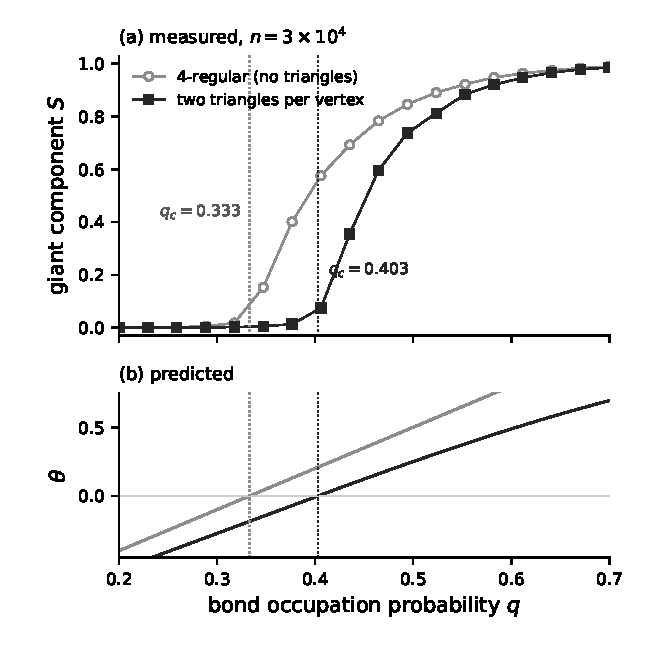
\includegraphics[width=0.86\linewidth]{figs/fig-triangles.pdf}
\caption{\textbf{Triangles hurt, at fixed degree.} Two networks with degree $4$
at every node and the same number of links; the only difference is that one has
its links arranged in triangles, giving clustering $1/3$ against $0$. (a) The
giant component measured by Monte Carlo. (b) The prediction, $\theta=3q-1$ and
$\theta=\bar s_{\triangle}(q)-1$. The measured onsets sit on the predicted
thresholds. Compare Eq.~\eqref{eq:deltatheta}, which finds the opposite sign at
fixed \emph{link count} --- because that comparison lets the degree distribution
broaden. Generated by \code{figs/\allowbreak triangles\_\allowbreak vs\_\allowbreak regular.\allowbreak py}.}
\label{fig:triangles}
\end{figure}

The mechanism is the one Chapter~\ref{ch:ising} will give for the Ising model,
in the form that covers both. A triangle transmits
\emph{more per neighbour} than a link does: at $q=1$ it delivers two nodes where
a link delivers one, and Eq.~\eqref{eq:thetaNM}'s $\bar s_{\triangle}$ exceeds
$\bar s_{|}$ at every $q$. But a node of degree four spends its four links on
two triangles rather than on four independent links, so it has \emph{two}
branches to explore instead of four. More per branch, fewer branches --- and the
second effect is the larger. That sentence, with $\bar s$ replaced by the
transmission of a magnetisation, is Chapter~\ref{ch:ising}'s headline result.

\section{Checks}
\label{sec:percolation-checks}

\checkhead{Known results}
Every specialisation in Sec.~\ref{sec:structurebystructure} reproduces a
published formula --- Molloy--Reed, Callaway \emph{et al.}, the hypergraph
result, \citeauthor{sun2021}'s multiplex expression. This tests the algebra and
nothing else.

\checkhead{New results}
Section~\ref{sec:helporhurt} is the only part of the chapter with no published
counterpart. Its two thresholds, $q_{c}=1/3$ for the $4$-regular graph and
$q_{c}=0.4030$ for the network of triangles, are confirmed by Monte Carlo on
both structures at $n=3\times10^{4}$ (Fig.~\ref{fig:triangles}): the measured
onsets sit on the predicted thresholds.

\checkhead{Partial results}
Sampling a chygraph from the configuration-model construction of
Sec.~\ref{sec:sampling} and percolating it tests the map, and not the assumption
the map rests on, because a chygraph built that way has complexes meeting in at
most one atom by construction. Figure~\ref{fig:triangles} is halfway past that:
the two-triangles-per-vertex network is a real graph, but it too was built with
the triangles sharing at most one atom. Nothing in this chapter needed the
complexes to be small, or the layers to be few, or the cardinality distribution
to be narrow; what it needed was that single assumption, and no check here tests
it. Building a structure where complexes share more is
Chapter~\ref{ch:overlap}'s business, and there the theory is not exact.
